% ------------------------------------------------------------------------
%  Instituto Mauá de Tecnologia
%  Núcleo de Sistemas Eletrônicos Embarcados - NSEE
%   Juliano Tusi Amaral Laganá Pinto
% 					 julianotusi@gmail.com
%  		
%  Projeto CITAR
%	Meta 4
% 	Especificação do produto
% 	Acionamento motor BLDC para rodas de reação
%
%	Outubro de 2014
% ------------------------------------------------------------------------
% ------------------------------------------------------------------------
% Modelo criado por: Rodrigo Romano
% "Rafael Corsi" <corsiferrao@gmail.com>
% ------------------------------------------------------------------------

%\documentclass[12pt,a4paper,twoside=semi, headinclude]{scrreprt}
\documentclass[
    fontsize=12pt,          % fontsize
    paper=a4,               % page size a4
    firsthead=on,           % display header on first page
    firstfoot=on,           % display footer on first page
    pagenumber=off,         % position of the page number
    parskip=half,           % Use indent instead of skip, half, false
    enlargefirstpage=on,    % more space on first page
    fromalign=left,         % placement of name in letter head
    fromrule=afteraddress,  % separate the address with a line in letter head, false or aftername
    fromemail=off,          % turn on email of sender
    fromurl=off,            % print URL of sender
    fromphone=off,          % turn on phone of sender
    fromlogo=off,           % turn on logo of sender
    addrfield=on,           % address field for envelope with window, on or true
    subject=titled,         % placement of subject, beforeopening or titled
    foldmarks=off,          % print foldmarks
    numericaldate=off,      % display date in numbers only
    KOMAold]{scrreprt}
%\usepackage[a4paper,left=3.5cm,right=1.5cm,top=3cm,bottom=2.5cm]{geometry}

\usepackage[utf8]{inputenc}       %Permite acentuação
\usepackage[T1]{fontenc}
\usepackage[english,brazil,brazilian]{babel}
\usepackage[centertags]{amsmath}



% ------------------------------------------------------------------------
\usepackage[automark,headsepline]{scrlayer-scrpage}
%\clearpairofpagestyles
\cfoot[\pagemark]{\pagemark}
\lehead{\headmark}
\rohead{\headmark}
\cfoot[\raisebox{-0.5em}{ -- \, \textnormal{\thepage} \, --}]{\raisebox{-0.5em}{ -- \, \textnormal{\thepage} \, --}}
\pagestyle{scrheadings}
%\include{authorpart}
% ------------------------------------------------------------------------

\usepackage{lmodern,
			url,
			hyperref,
			multirow,
			array,
			indentfirst,
			ncccomma,
			pst-node,
			pstricks,
			schemabloc,
			amssymb,
			amsfonts,
			graphicx,
			etoolbox, 
			pdfpages,
			hyperref,
			paralist,
			tabularx,
			pdflscape,
			color,				
			doc,
			vhistory,
			tcolorbox,
			titlepic,
			hyperref}
			
\usepackage[titletoc,toc,title]{appendix}
% ------------------------------------------------------------------------
% Reduz espacamento na bibliografia
%\usepackage{natbib}
%\setlength{\bibsep}{0.0pt}

%Matem figura na secção !
%\usepackage[section]{placeins}

% sub figuras
%ajuste do tamanho entre figuras
\usepackage{subfigure}
\setlength\subfigcapmargin{0.8em}

% Fuzz 
\hfuzz1pt % Don't bother to report over-full boxes if over-edge is < 2pt

% Numeração das notas de rodapé 
\renewcommand{\thefootnote}{\fnsymbol{footnote}}

% Different font in captions 
\newcommand{\captionfonts}{\small}

\makeatletter  % Allow the use of @ in command names
\long\def\@makecaption#1#2{%
  \vskip\abovecaptionskip
  \sbox\@tempboxa{{\captionfonts #1: #2}}%
  \ifdim \wd\@tempboxa >\hsize
    {\captionfonts #1: #2\par}
  \else
    \hbox to\hsize{\hfil\box\@tempboxa\hfil}%
  \fi
  \vskip\belowcaptionskip}
\makeatother   % Cancel the effect of \makeatletter

% Espaçamento
\setlength{\parindent}{30pt} \setlength{\parskip}{6pt}
\newlength{\defbaselineskip}
\setlength{\defbaselineskip}{\baselineskip}

\newcommand{\setlinespacing}[1]{\setlength{\baselineskip}{#1 \defbaselineskip}}
% ---
\newcommand{\PreserveBackslash}[1]{\let\temp=\\#1\let\\=\temp}
\let\PBS=\PreserveBackslash %
\def\baselinestretch{1}
\setlinespacing{1.5}
% ------------------------------------------------------------------------
% Use the microtype package for better typography
% http://www.khirevich.com/latex/microtype/
%
% activate={true,nocompatibility} - activate protrusion and expansion
% final - enable microtype; use "draft" to disable
% tracking=true, kerning=true, spacing=true - activate these techniques
% factor=1100 - add 10% to the protrusion amount (default is 1000)
% stretch=10, shrink=10 - reduce stretchability/shrinkability (default is 20/20)
\usepackage[activate={true,nocompatibility},
			final,
			tracking=true,
			kerning=true,
			spacing=true,
			factor=1100,
			stretch=10,
			shrink=10]
			{microtype} 

% Possibilita que caracteres saiam da margem p/ melhor caber o texto
\SetProtrusion{encoding={*},
			   family={bch},
			   series={*},size={6,7}}
               {1={ ,750},2={ ,500},3={ ,500},4={ ,500},5={ ,500},
               6={ ,500},7={ ,600},8={ ,500},9={ ,500},0={ ,500}}

\microtypecontext{spacing=nonfrench}
% ------------------------------------------------------------------------
               
% Todo notes
%\usepackage[disable]{todonotes}
\usepackage[colorinlistoftodos]{todonotes}  
\setlength{\marginparwidth}{2cm}
\reversemarginpar             
%\makeatletter\let\chapter\@undefined\makeatother

\newcommand\todoin[2][]{\todo[inline, caption={2do}, #1, color={red!100!green!33}]{
\begin{minipage}{\textwidth-4pt}#2\end{minipage}}}

% ------------------------------------------------------------------------

% Restora contagem da nota a cada pagina
\usepackage{perpage}
\MakePerPage{footnote}

% Qualidade e compressão do pdf
%\pdfminorversion=5
%\pdfcompresslevel=9
%\pdfobjcompresslevel=2

% ------------------------------------------------------------------------
% Possibilita inserir pdf com texto fora do arquivo
% util para figs geradas no inkscape
\newcommand{\executeiffilenewer}[3]{%
\ifnum\pdfstrcmp{\pdffilemoddate{#1}}%
{\pdffilemoddate{#2}}>0%
{\immediate\write18{#3}}\fi%
}

\newcommand{\includesvg}[1]{%
\executeiffilenewer{#1.svg}{#1.pdf}%
{inkscape -z -D --file=./Figs/#1.svg %
--export-pdf=./Figs/#1.pdf --export-latex}%
\input{./figs/#1.pdf_tex}%
}
\usepackage{natbib}
%------------------------------------------------------------------------	
\usepackage{tikz}
\graphicspath{ {./figs/} }
% ------------------------------------------------------------------------
\newtcolorbox[auto counter,number within=section]{TBD-BOX}[2][]{%
colback=red!5!white,colframe=darkgray,fonttitle=\bfseries,
title=TBD.~\thetcbcounter: #2,#1}
% ------------------------------------------------------------------------
% http://latexcolor.com/
% cores dos todos
\definecolor{TBC}{rgb}{0.98, 0.91, 0.71}  	%bananamania
\definecolor{Corsi}{rgb}{0.53, 0.66, 0.42}  %
%\definecolor{TBC2}{rgb}{1.0, 0.71, 0.76} 		%lightpink
\definecolor{TBC2}{rgb}{0.86, 0.82, 1.0} %lightmauve
\definecolor{darkgray}{rgb}{0.66, 0.66, 0.66}
\definecolor{aliceblue}{rgb}{0.94, 0.97, 1.0}
% ------------------------------------------------------------------------

\title		{   \LARGE
				Instituto Mauá de Tecnologia \\
				Núcleo de Sistemas Eletrônicos Embarcados - NSEE \\
				\vspace{10px}
				\huge
				Simulador motor BLDC \\
			}
\author		{
				 Juliano Tusi Amaral Laganá Pinto \\ \small 	
				\href{mailto:julianotusi@gmail.com}{julianotusi@gmail.com}
			}
%\subject	{Núcleo de Sistemas Eletrônicos Embarcados - NSEE}			
\titlepic	{
\includegraphics[width=0.4\textwidth]{maua_logo}}
%\lowertitleback{}

% ------------------------------------------------------------------------
\begin{document}
% ------------------------------------------------------------------------
\maketitle
\tableofcontents
% ------------------------------------------------------------------------
%%---------- Revisão
\begin{versionhistory}
  \vhEntry{1.0.0}{16.10.14}{Juliano Laganá}{Criação do documento.}
  \vhEntry{1.0.1}{21.10.14}{Juliano Laganá}{Adição do encoder e do método M/T aos blocos especificados.}
  \vhEntry{1.0.2}{24.06.15}{Juliano Laganá}{Substituição do modelo elétrico de fases individuais pelo modelo elétrico com as fases acopladas.}
  \vhEntry{1.0.3}{24.06.15}{Juliano Laganá}{Adição do bloco de conversão de tensões.}
  \vhEntry{1.0.4}{24.06.15}{Juliano Laganá}{Correção da definição do parâmetro L. Na verdade é a indutância por fase descontada da indutância mútua.}
  \vhEntry{1.0.5}{25.06.15}{Juliano Laganá}{Inclusão do modelo de atrito de Coulomb}
\end{versionhistory}



\chapter{Introdução}

    \section{Objetivo}
        O objetivo desse documento é disponibilizar um manual de uso da biblioteca ``BLDC.slx'' para simulação do motor DC sem escovas (BLDC).

    \section{Sistema de interesse}
        O sistema de interesse é um motor DC sem escovas acoplado à uma carga constante. A figura \ref{fig_modelo_simplificado} ilustra um modelo simplificado do sistema. Os torques mostrados no desenho são:
        \begin{itemize}
            \item $T_e$ : Torque elétrico gerado pelo motor.
            \item $T_d$ : Torque de atrito no mancal (atrito viscoso + atrito de Coulomb).
            \item $T_l$ : Torque da carga.
        \end{itemize}

        \begin{figure}[ht]
            \centering
            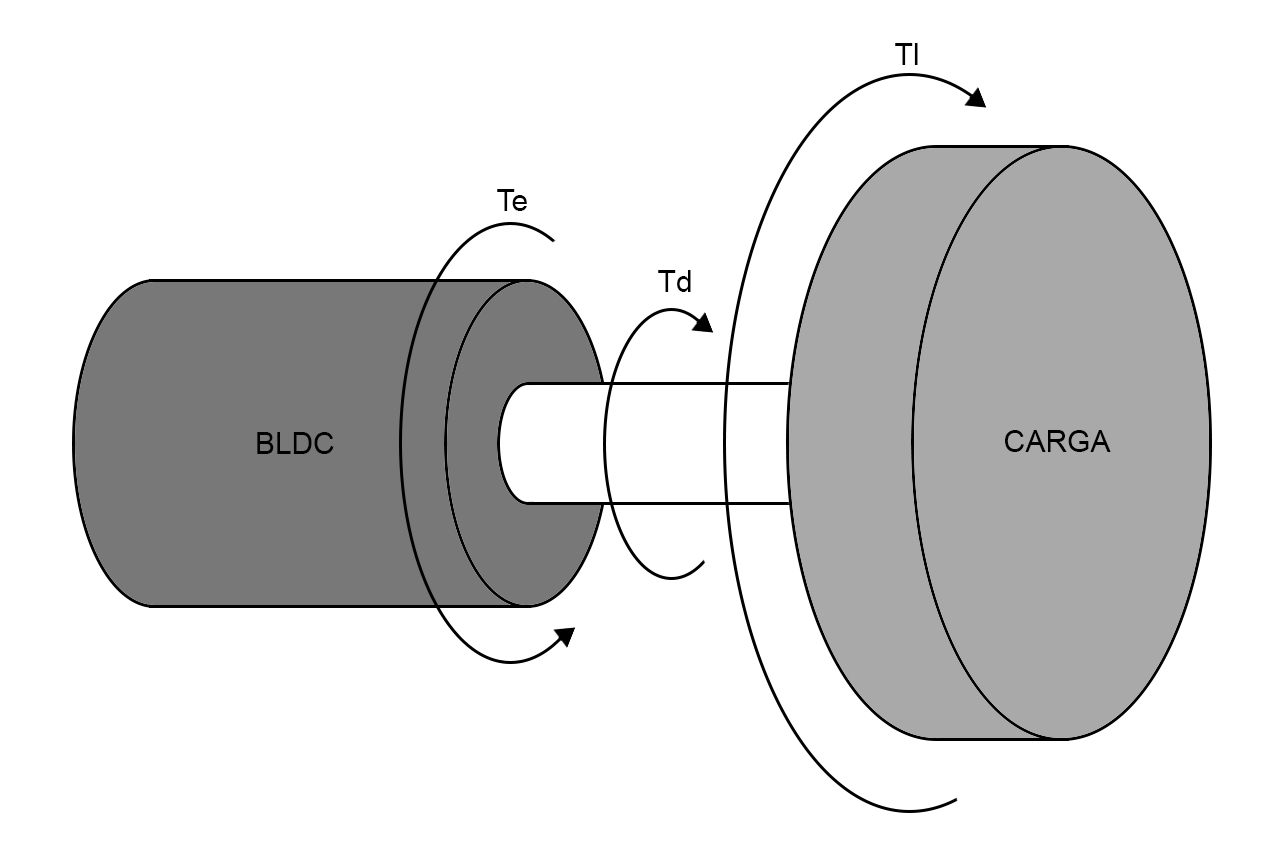
\includegraphics[width=0.7\textwidth]{sketch_bldc}
            \caption{Modelo simplificado do sistema}
            \label{fig_modelo_simplificado}
        \end{figure}

    \section{Hipóteses}
        \begin{itemize}
            \item Todas as fases de alimentação do BLDC tem a mesma resistência.
            \item Todas as fases de alimentação do BLDC tem a mesma indutância.
            \item Todos as partes do sistema são consideradas corpos rígidos.
            \item O atrito no mancal pode ser modelado como atrito viscoso (diretamente proporcional à velocidade angular do rotor em relação ao estator) + atrito de Coulomb.
            \item A força contraeletromotriz gerada em cada fase de alimentação tem o formato trapezoidal.
        \end{itemize}

    \section{Modelo matemático}
    \label{sec:modelo_matematico}
        \begin{itemize}
            \item Dinâmica mecânica, com atrito viscoso e atrito de Coulomb: 
                $$J.\frac{d^2\theta_m}{dt^2}=T_e-T_l-T_{at1}-T_{at2}$$
                $$T_{at1} = K_d.\frac{d\theta_m}{dt}$$
                 \begin{displaymath}
                   T_{at2} = \left\{
                     \begin{array}{lr}
                       -T_k.sign(\frac{d\theta}{dt}) & : \frac{d\theta_m}{dt} \neq 0\\
                       -min(T_s,T_e-T_l).sign(T_e-T_l) & : \frac{d\theta_m}{dt} = 0
                     \end{array}
                   \right.
                \end{displaymath}
            \item Dinâmica elétrica, como proposto por \cite{baldursson}:
                $$v_{ab} = R(i_a-i_b)+L\frac{d}{dt}(i_a-i_b)+e_a-e_b$$
                $$v_{bc} = R(i_a+2i_b)+L\frac{d}{dt}(i_a+2i_b)+e_b-e_c$$
                $$i_a+i_b+i_c=0$$
            \item Forças contraeletromotrizes geradas em cada fase:
                $$e_a = \frac{f_a(\theta_e).K_e}{2}.\frac{d\theta_m}{dt} $$
                $$e_b = \frac{f_b(\theta_e).K_e}{2}.\frac{d\theta_m}{dt} $$
                $$e_c = \frac{f_c(\theta_e).K_e}{2}.\frac{d\theta_m}{dt} $$
            \item Torque gerado por cada fase e torque elétrico total:
                $$T_a=\frac{f_a(\theta_e).K_t.i_a}{2}$$
                $$T_b=\frac{f_b(\theta_e).K_t.i_b}{2}$$
                $$T_c=\frac{f_c(\theta_e).K_t.i_c}{2}$$
                $$T_e=T_a+T_b+T_c$$
            \item Relação entre ângulo elétrico e ângulo mecânico:
                $$\theta_e=\theta_m.\frac{P}{2}$$
        \end{itemize}

        \begin{description}
            \item[$J$] = Inércia do sistema motor+carga
            \item[$K_d$] = Coeficiente de atrito viscoso do mancal
            \item[$T_{at1}$] = Torque devido ao atrito viscoso
            \item[$T_{at2}$] = Torque devido ao atrito de Coulomb
            \item[$T_k$] = Magnitude do torque devido ao atrito cinético
            \item[$T_s$] = Magnitude máxima do torque devido ao atrito estático
            
            \item[$K_e$] = Constante de força contraeletromotriz
            \item[$K_t$] = Constante de torque
            \item[$P$] = Número de pólos

            \item[$\theta_m$] = Ângulo do rotor em relação ao estator
            \item[$\theta_e$] = Ângulo elétrico

            \item[$L$] = Indutância de cada fase (descontada do valor da indutância mútua, caso seja significativo)
            \item[$R$] = Resistência de cada fase
            \item[$v_{ab}$] = Tensão entre as fase $a$ e $b$
            \item[$v_{bc}$] = Tensão entre as fases $b$ e $c$
            \item[$i_a$] = Corrente na fase $a$
            \item[$i_b$] = Corrente na fase $b$
            \item[$i_c$] = Corrente na fase $c$
            \item[$e_a$] = Força contraeletromotriz gerada na fase $a$
            \item[$e_b$] = Força contraeletromotriz gerada na fase $b$
            \item[$e_c$] = Força contraeletromotriz gerada na fase $c$
            \item[$T_a$] = Torque elétrico gerado pela fase $a$ no rotor
            \item[$T_b$] = Torque elétrico gerado pela fase $b$ no rotor
            \item[$T_c$] = Torque elétrico gerado pela fase $c$ no rotor
            \item[$T_e$] = Torque elétrico total aplicado no rotor

            \item[$f_a(\theta_e)$] = Função que reproduz o comportamento trapezoidal da força contraeletromotriz na fase $a$
            \item[$f_b(\theta_e)$] = Função que reproduz o comportamento trapezoidal da força contraeletromotriz na fase $b$
            \item[$f_c(\theta_e)$] = Função que reproduz o comportamento trapezoidal da força contraeletromotriz na fase $c$
            
            \item[$sign(x)$] = Retorna 1 se $x$ é não-negativo, $-1$ caso contrário.
            \item[$min(a,b)$] = Retorna $a$ se $a>b$, $b$ caso contrário. 


        \end{description}

\chapter{Implementação}

    \section{Bloco BLDC}
        O modelo matemático apresentado na seção \ref{sec:modelo_matematico} foi implementado no bloco ``BLDC'' ilustrado na figura \ref{fig:bloco_BLDC}. Todos os parâmetros do motor podem ser alterados clicando-se duas vezes em cima do bloco.
        \begin{figure}[ht]
            \centering
            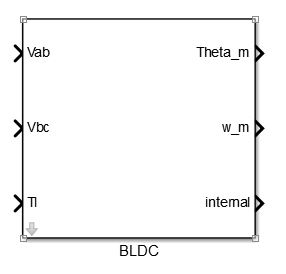
\includegraphics[width=0.3\textwidth]{bloco_BLDC}
            \caption{Bloco simulink para simulação do BLDC}
            \label{fig:bloco_BLDC}
        \end{figure}

        \begin{itemize}
            \item Entradas
            \begin{enumerate}
                \item Vab - Tensão entre as fases $a$ e $b$ [V]
                \item Vbc - Tensão entre as fases $b$ e $c$ [V]
                \item Tl - Torque da carga [N.m]
            \end{enumerate}
            \item Saídas
            \begin{enumerate}
                \item Theta\_m - Ângulo entre o rotor e o estator ($\theta_m$) [rad]
                \item w\_m - Velocidade angular entre o rotor e o estator ($\frac{d\theta_m}{dt}$) [rad/s]
                \item internal - Sinal multiplexado [4x1] composto pelos seguintes sinais:
                \begin{itemize}
                    \item Correntes [3x1] - $i_a$, $i_b$ e $i_c$ [A]
                    \item Torques [3x1] - $T_a$, $T_b$ e $T_c$ [N.m]
                    \item FCEMs [3x1] - $e_a$, $e_b$ e $e_c$ [V]
                    \item Torque total - $T_e$ [N.m]
                    \item Torque de atrito - $T_{at2}$
                \end{itemize}
            \end{enumerate}
        \end{itemize}

    \section{Bloco BLDC com lógica de comutação em blocos}
        Para o devido funcionamento do BLDC é necessário comutar a tensão entre cada fase periodicamente. O bloco apresentado na figura \ref{fig:bloco_BLDC_block_commutation} implementa internamente a estratégia de comutação em blocos através da utilização de três sensores de efeito hall separados por 120 graus. Todos os parâmetros do motor podem ser alterados clicando-se duas vezes em cima do bloco.
        \begin{figure}[ht]
            \centering
            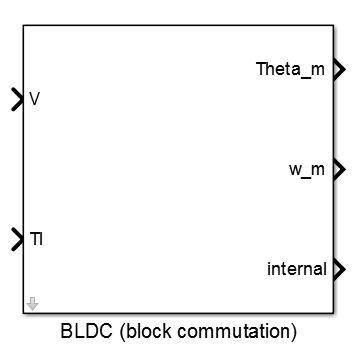
\includegraphics[width=0.3\textwidth]{bloco_BLDC_block_commutation}
            \caption{Bloco simulink para simulação do BLDC utilizando comutação em blocos}
            \label{fig:bloco_BLDC_block_commutation}
        \end{figure}

        \begin{itemize}
            \item Entradas
            \begin{enumerate}
                \item V - Tensão aplicada nas fases [V]
                \item Tl - Torque da carga [N.m]
            \end{enumerate}
            \item Saídas
            \begin{enumerate}
                \item Theta\_m - Ângulo entre o rotor e o estator ($\theta_m$) [rad]
                \item w\_m - Velocidade angular entre o rotor e o estator ($\frac{d\theta_m}{dt}$) [rad/s]
                \item internal - Sinal multiplexado [4x1] composto pelos seguintes sinais:
                \begin{itemize}
                    \item Correntes [3x1] - $i_a$, $i_b$ e $i_c$ [A]
                    \item Torques [3x1] - $T_a$, $T_b$ e $T_c$ [N.m]
                    \item FCEMs [3x1] - $e_a$, $e_b$ e $e_c$ [V]
                    \item Torque total - $T_e$ [N.m]
                    \item Hall [3x1] - $H_1$, $H_2$ e $H_3$ (Níveis lógicos de cada sensor Hall acoplado ao motor)
                \end{itemize}
            \end{enumerate}
        \end{itemize}

\chapter{Ferramentas adicionais}

    \section{Conversão de tensões}
        Foi desenvolvido um bloco para converter as tensões individuais de cada fase ($V_a$, $V_b$ e $V_c$) nas tensões entre as fases ($v_ab$ e $v_bc$, que são as entradas do bloco BLDC), ilustrado na figura \ref{fig:bloco_conversao_tensoes}.
        \begin{figure}[ht]
            \centering
            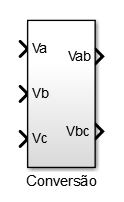
\includegraphics[width = 0.15\textwidth]{bloco_conversao_tensoes}
            \caption{Bloco para converter as tensões individuais em tensões entre fases}
            \label{fig:bloco_conversao_tensoes}
        \end{figure}

        \begin{itemize}
            \item Entradas
                \begin{enumerate}
                    \item $Va$ - Tensão na fase $a$
                    \item $Vb$ - Tensão na fase $b$
                    \item $Vc$ - Tensão na fase $c$
                \end{enumerate}
            \item Saídas
                \begin{enumerate}
                    \item $v_{ab}$ - Tensão entre as fases $a$ e $b$
                    \item $v_{bc}$ - Tensão entre as fases $b$ e $c$
                \end{enumerate}
        \end{itemize}

    \newpage
    \section{Medição de posição}
        Para medição de posição angular do rotor foi desenvolvido um bloco que simula o funcionamento de um encoder de quadratura, ilustrado na figura \ref{fig:bloco_encoder}. O número de pulsos por revolução pode ser configurado clicando-se duas vezes no bloco.
        \begin{figure}[ht]
            \centering
            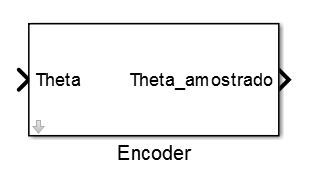
\includegraphics[width=0.3\textwidth]{bloco_encoder}
            \caption{Bloco simulink para simulação de um encoder de quadratura}
            \label{fig:bloco_encoder}
        \end{figure}

        \begin{itemize}
            \item Entradas
                \begin{enumerate}
                    \item Theta - Ângulo mecânico entre o rotor e o estator. [graus]
                \end{enumerate}
            \item Saídas
                \begin{enumerate}
                    \item Theta\_amostrado - Ângulo mecânico entre o rotor e o estator, amostrado pelo encoder de quadratura simulado. [graus]
                \end{enumerate}
            \item Restrições
                \begin{enumerate}
                    \item Para o correto funcionamento desse bloco, o step size da simulação deve ser configurado para nunca exceder $\frac{360}{4.N_r.V_{máx}}$ segundos; onde $N_r$ é o número de pulsos por rotação do encoder (especificado clicando-se duas vezes em cima do bloco) e $V_{máx}$ é o valor máximo da derivada da entrada Theta em graus/s. Exemplo: Para a correta simulação de um encoder com $N_r=300$, amostrando um BLDC cuja velocidade angular atinge no máximo $1200$ graus/s (portanto o valor máximo da derivada da entrada Theta também é $1200$ graus/s), faz-se necessário configurar a simulação para que o step size nunca exceda $2,5 . 10^{-4}$ segundos.
                \end{enumerate}
        \end{itemize}


    \newpage
    \section{Medição de velocidade}
        O algoritmo M/T para estimação de velocidade \cite{algoritmoMT} foi implementado no simulink e está ilustrado na figura \ref{fig:bloco_MT}
        \begin{figure}[ht]
            \centering
            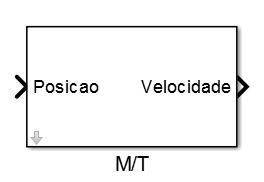
\includegraphics[width=0.3\textwidth]{bloco_MT}
            \caption{Bloco que implementa o algoritmo de estimação de velocidade M/T}
            \label{fig:bloco_MT}
        \end{figure}

        \begin{itemize}

            \item Entradas
                \begin{enumerate}
                    \item Posicao - Essa entrada deve ser conectada à saída ``Theta\_amostrado'' do bloco simulador de encoder de quadratura. [graus]
                \end{enumerate}
            \item Saídas
                \begin{enumerate}
                    \item Velocidade - Velocidade estimada pelo algorimo M/T. [graus/s]
                \end{enumerate}
        \end{itemize}




\bibliographystyle{plain}
\bibliography{bibfile}


\end{document}
